ubuntu系统为我们提供了完整的图形化界面,大部分操作已经可以通过图形化界面来完成,但如何通过命令行来和linux系统进行交互仍是基本功,下面我们就来简单介绍一下linux系统的基本操作。
\subsubsection{linux文件系统基本概念}
\textbf{linux目录结构}

首先我们来看一下linux系统的树状目录结构:

\begin{figure}[H]
    \centering
    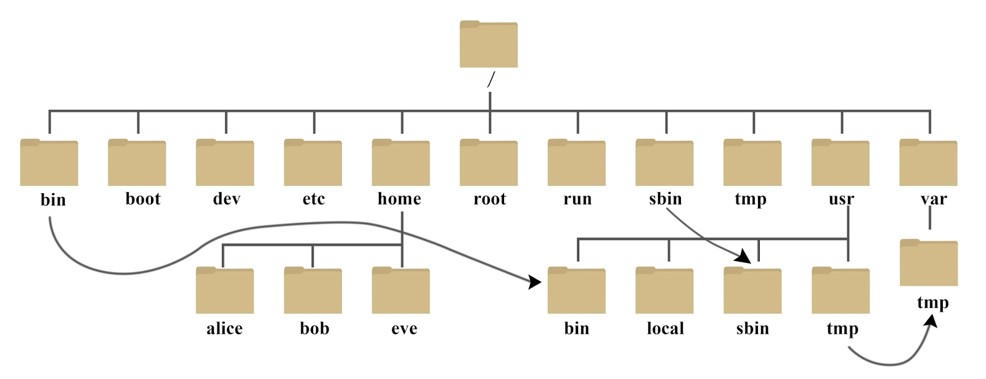
\includegraphics[width=0.9\textwidth]{linux7.jpg}
    \caption{linux系统树状目录结构} % 图片标题
    \label{fig:linux7} % 图片标签,用于引用
\end{figure}

可以看到整个linux系统是由若干个文件夹反复嵌套组成的,目录结构如同一棵倒置的树,因此最上面的文件夹被称为“根目录”。

\textbf{“一切皆文件”}

在linux系统中有一个非常重要的、区别于windows系统的概念是“一切皆文件”,也就是把一切资源都看作是文件,包括硬件设备(通常称为设备文件),这样好处是用户可以用读写文件的方式实现对硬件的访问。举个简单的例子:假如现在将U盘插到电脑上,在windows上会看到出现一个新的磁盘,在linux中则可以在/dev目录下找到新出现的文件夹,该文件夹中就存放了插入U盘的相关内容,用户不仅可以修改U盘中存储的文件,还可以修改其相关配置。

\textbf{挂载}

在上述例子中,U盘与linux系统建立连接的过程称为“挂载”。Linux系统中没有磁盘分区的逻辑概念,任何一个种类的文件系统被创建后,都需要挂载到某个特定的目录才能使用,这个过程相当于激活一个文件系统,使它能够使用。简单来说“挂载”就是将linux本身文件目录与硬件设备的文件目录合二为一,下图中展示了一个简单的挂载实例。

\begin{figure}[H]
    \centering
    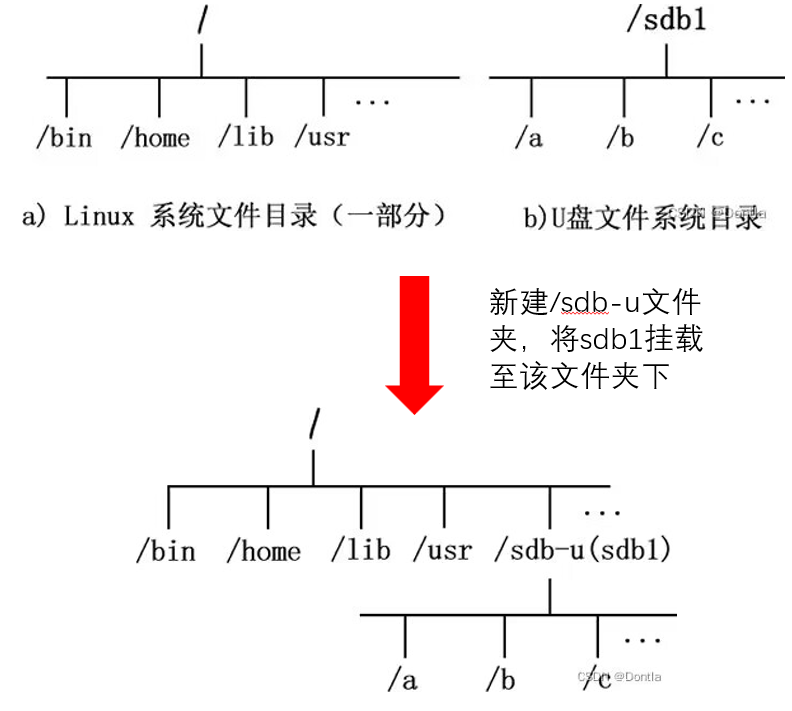
\includegraphics[width=0.7\textwidth]{linux8.png}
    \caption{挂载实例} % 图片标题
    \label{fig:linux8} % 图片标签,用于引用
\end{figure}

Windows的文件系统挂载使用其内部机制完成,用户基本无法探知其过程。而Linux使用mount工具对文件系统进行挂载。挂载文件系统时,需要明确挂载点,在创建文件系统后,操作系统会提示将此文件系统挂载至哪个位置,这个位置就是挂载点,通常选择“/”即根目录。挂载操作在备份系统镜像时经常用到。

\textbf{主要文件夹及其作用}

/bin:bin 是 Binaries (二进制文件) 的缩写, 这个目录存放着最经常使用的命令。

/boot:这里存放的是启动 Linux 时使用的一些核心文件,包括一些连接文件以及镜像文件。

/dev:dev 是 Device(设备) 的缩写, 该目录下存放的是 Linux 的外部设备,在 Linux 中访问设备的方式和访问文件的方式是相同的。

/etc:etc 是 Etcetera(等等) 的缩写,这个目录用来存放所有的系统管理所需要的配置文件和子目录。

/home:用户的主目录,在 Linux 中,每个用户都有一个自己的目录,一般该目录名是以用户的账号命名的,如上图中的 alice、bob 和 eve。

/lib:lib 是 Library(库) 的缩写这个目录里存放着系统最基本的动态连接共享库,其作用类似于 Windows 里的 DLL 文件。几乎所有的应用程序都需要用到这些共享库。

/opt:opt 是 optional(可选) 的缩写,这是给主机额外安装软件所摆放的目录。比如你安装一个ORACLE数据库则就可以放到这个目录下。默认是空的。

/root:该目录为系统管理员,也称作超级权限者的用户主目录。

/usr:usr 是 unix system resources(unix 系统资源) 的缩写,这是一个非常重要的目录,用户的很多应用程序和文件都放在这个目录下,类似于 windows 下的 program files 目录。

/var:var 是 variable(变量) 的缩写,这个目录中存放着在不断扩充着的东西,我们习惯将那些经常被修改的目录放在这个目录下。包括各种日志文件。

在这些文件夹中,/bin,/etc,/usr,/var内存放着重要的系统文件,如果删除可能会导致系统出错,因此在平时操作时要多加注意。

\subsubsection{linux系统基本操作}
由于篇幅有限,本部分仅能列出平时操作中最常用的部分,其它内容如需用到请读者自行查阅资料。

\textbf{01用户管理}
\begin{table}[!htbp]
	\centering
	\begin{tabular}{cc}
		\toprule[1.5pt]
		命令 & 作用\\
		\midrule[1pt]
		$id \enspace [name]$			&查看用户UID和GID信息\\
		$who$			&查看当前所有登录的用户列表\\
		$whoami$			&查看当前登录用户的账户名\\
		$su \enspace -[name]$			&切换用户,并且切换目录\\
		$exit$			&退出当前登录用户\\
		$passwd\enspace [name]$			&设置用户密码\\
		\bottomrule[1.5pt]
	\end{tabular}
\end{table}

说明:
\begin{enumerate}
	\item -\enspace 可以切换到用户家目录,否则保持位置不变
	\item su 不接用户名,可以切换到 root 
	\item 命令前加sudo:以超级用户权限运行命令
\end{enumerate}

\textbf{02系统信息}

\begin{table}[!htbp]
	\centering
	\begin{tabular}{cc}
		\toprule[1.5pt]
		语法 & 作用\\
		\midrule[1pt]
		$free\enspace -m$			&以MB为单位显示系统内存使用情况\\
		$uname \enspace -amnrsv \enspace --help \enspace --version$			&显示电脑以及操作系统的相关信息\\
		\bottomrule[1.5pt]
	\end{tabular}
\end{table}

\begin{center}
\textbf{uname参数说明}

	\begin{tabular}{cc}
		\toprule[1.5pt]
		参数 & 作用\\
		\midrule[1pt]
		$-a\enspace --all$		&显示全部的信息\\
		$-m\enspace --machine $		&显示处理器类型\\
		$-n\enspace --nodename $		&显示主机名\\
		$-r\enspace --release $		&显示内核版本号\\
		$-s\enspace --sysname $		&显示操作系统名称\\
		$-v $		&显示操作系统的版本\\
		$--help $		&显示帮助\\
		$--version $		&显示版本信息\\
		$-p $		&显示处理器类型(与 -m 选项相同)\\
		\bottomrule[1.5pt]
	\end{tabular}
\end{center}

\textbf{03软件安装}

软件安装命令有yum,apt等等,比较常用的是apt,apt 命令执行需要超级管理员权限

\begin{table}[!htbp]
	\centering
	\begin{tabular}{cc}
		\toprule[1.5pt]
		语法 & 作用\\
		\midrule[1pt]
		$  apt\enspace [options] \enspace [command] \enspace [package ...]$		&查找、安装、升级、删除软件包\\
		\bottomrule[1.5pt]
	\end{tabular}
\end{table}

\textbf{options}:可选,选项包括 -h(帮助),-y(当安装过程提示选择全部为"yes"),-q(不显示安装的过程)等等

\textbf{command}:要进行的操作

\textbf{package}:安装的包名\\

\begin{center}
\textbf{apt常用命令如下}

	\begin{tabular}{cc}
		\toprule[1.5pt]
		命令 & 作用\\
		\midrule[1pt]
		$  apt\enspace update$	&列出所有可更新的软件清单\\
		$  apt\enspace upgrade$	&升级软件包\\
		$  apt\enspace list \enspace --upgradable$		&列出可更新的软件包及版本信息\\
		$  apt\enspace full-upgrade$	&升级软件包前先删除需要更新软件包\\
		$  apt\enspace install \enspace \textless package1\textgreater \enspace \textless package2\textgreater $	&安装指定的软件\\
		$  apt\enspace update \enspace \textless package\textgreater $		&更新指定的软件\\
		$  apt\enspace show \enspace \textless package\textgreater $	&显示软件包具体信息\\
		$  apt\enspace remove \enspace \textless package\textgreater $		&删除软件包\\
		$  apt\enspace autoremove$		&清理不再使用的依赖和库文件\\
		$  apt\enspace purge \textless package\textgreater $		&移除软件包及配置文件\\
		$  apt\enspace search \enspace \textless keyword\textgreater $		&找软件包命令\\
		$  apt\enspace list \enspace --installed$		&列出所有已安装的包\\
		$  apt\enspace list \enspace --all-versions$	&列出所有已安装的包的版本信息\\
		\bottomrule[1.5pt]
	\end{tabular}
\end{center}

\textbf{04文件与目录管理}

首先先介绍一些常用概念

\begin{enumerate}
\item 绝对路径:路径的写法,由根目录\enspace /\enspace 写起,例如:/usr/share/doc 这个目录。
\item 相对路径:路径的写法,相对于当前所处的文件夹位置,不是由\enspace /\enspace 写起,例如由 /usr/share/doc 要到 /usr/share/man 底下时,可以写成:cd man
\item \enspace .\enspace :在相对路径中使用,表示当前目录
\item \enspace ..\enspace :在相对路径中使用,表示上一级目录
\item \enspace *\enspace :通配符,可以代表文件名中的任意字符或字符串,但不能与句点打头的文件名匹配
\item 文件类型:分为目录(d),文件(-),链接文件(l),装置文件里可供储存的接口设备(b),装置文件里面的串行端口设备(c)
\item 文件基本属性:分为可读(r),可写(w),可执行(x)。Linux文件属性有两种设置方法,一种是数字,一种是符号。使用数字来代表各个权限时,各权限的分数对照为:r:4,w:2,x:1
\end{enumerate}

处理文件和目录的命令有很多,这里分表整理了一些常用命令的语法及其选项和参数仅供大家参考

\begin{center}
\textbf{常用处理文件和目录的命令}

	\begin{tabular}{cc}
		\toprule[1.5pt]
		语法 & 作用\\
		\midrule[1pt]
		$  ls$		&列出当前目录中的文件和子目录\\
		$  pwd$		&显示当前工作目录的路径\\
		$  cd\enspace /path/to/directory$		&切换工作目录\\
		$  mkdir\enspace [directory]$		&创建新目录\\
		$  cp\enspace [source]\enspace [destination]$		&复制文件或目录\\
		$  rm\enspace [file name]$		&删除文件或目录\\
		$  mv\enspace [old]\enspace [new]$		&移动或重命名文件或目录\\
		$  chmod\enspace [permissions]\enspace [file name]$		&修改文件或目录的权限\\
		$  tar\enspace [options]\enspace -f\enspace archive.tar\enspace [files...]$	&解压或压缩文件或目录\\
		$  zip\enspace [options]\enspace output.zip\enspace [files...]$		&压缩文件或目录\\
		$ unzip archive.zip$		&解压文件或目录\\
		\bottomrule[1.5pt]
	\end{tabular}
\end{center}

\begin{center}
\textbf{ls\enspace 选项和参数}

	\begin{tabular}{cc}
		\toprule[1.5pt]
		参数 & 作用\\
		\midrule[1pt]
		$  -a $		&列出当前目录中全部的文件,包括隐藏文件\\
		$  -d $		&仅列出目录本身,而不是列出目录内的文件数据\\
		$  -l $		&长数据串列出,包含文件的属性与权限等\\
		\bottomrule[1.5pt]
	\end{tabular}
\end{center}

\begin{center}
\textbf{mkdir\enspace 选项和参数}

	\begin{tabular}{cc}
		\toprule[1.5pt]
		参数 & 作用\\
		\midrule[1pt]
		$  -m $		&配置文件的权限\\
		$  -p $		&递归创建所需目录\\
		\bottomrule[1.5pt]
	\end{tabular}
\end{center}

\begin{center}
\textbf{cp\enspace 选项和参数}

	\begin{tabular}{cc}
		\toprule[1.5pt]
		参数 & 作用\\
		\midrule[1pt]
		$  -a $		&相当于\enspace -pdr\enspace 的意思\\
		$  -d $		&若来源档为链接档的属性(link file),则复制链接档属性而非文件本身\\
		$  -f $		&强制,若目标文件已经存在且无法开启,则移除后再尝试一次\\
		$  -i $		&若目标文件或目录已经存在,在覆盖时会先询问用户\\
		$  -l $		&进行硬式链接的链接档创建,而非复制文件本身\\
		$  -p $		&连同文件的属性一起复制过去,而非使用默认属性(备份常用)\\
		$  -r $		&递归持续复制,用于目录的复制(常用)\\
		$  -s $		&复制成为符号链接档,即“捷径”文件\\
		$  -u $		&若 destination 比 source 旧才升级 destination\\
		\bottomrule[1.5pt]
	\end{tabular}
\end{center}

\begin{center}
\textbf{rm\enspace 选项和参数}

	\begin{tabular}{cc}
		\toprule[1.5pt]
		参数 & 作用\\
		\midrule[1pt]
		$  -f $		&强制的意思,如果目标文件已经存在,不会询问而直接覆盖\\
		$  -i $		&互动模式,在删除前会询问使用者是否动作\\
		$  -r $		&递归删除,常用在目录的删除\\
		\bottomrule[1.5pt]
	\end{tabular}
\end{center}

\begin{center}
\textbf{mv\enspace 选项和参数}

	\begin{tabular}{cc}
		\toprule[1.5pt]
		参数 & 作用\\
		\midrule[1pt]
		$  -f $		&强制的意思,如果目标文件已经存在,不会询问而直接覆盖\\
		$  -i $		&若目标文件已经存在时,会询问是否覆盖\\
		$  -u $		&若目标文件已经存在,且 source 比较新,才会升级 \\
		\bottomrule[1.5pt]
	\end{tabular}
\end{center}

\begin{center}
\textbf{chmod\enspace 选项和参数}

	\begin{tabular}{cc}
		\toprule[1.5pt]
		参数 & 作用\\
		\midrule[1pt]
		$  -R $		&进行递归的持续变更,连同次目录下的所有文件都会变更\\
		$  u $		&user,用户身份\\
		$  g $		&group,组 \\
		$  o $		&others,其他身份 \\
		$  a $		&all,全部的身份 \\
		$  +\enspace -\enspace = $		&对权限加入,除去,设定 \\
		\bottomrule[1.5pt]
	\end{tabular}
\end{center}

使用chmod命令修改文件或目录权限有两种方式,一是用权限数字更改,方法为:

chmod [-R] xyz 文件或目录

其中xyz就是刚刚提到的数字类型的权限属性,为 rwx 属性数值的相加。

第二种是用符号类型改变文件权限,方法为:

chmod\enspace ([身份])\enspace +/-/=\enspace [permissions]\enspace [file name]

举例:

chmod 777 filename    修改文件/目录权限为所有人可读可写可执行

chmod u+x ex1.py        为 ex1.py 文件拥有者增加可执行权限

\begin{center}
\textbf{tar\enspace 选项和参数}

	\begin{tabular}{cc}
		\toprule[1.5pt]
		参数 & 作用\\
		\midrule[1pt]
		$  -f\enspace archive.tar $		&指定归档文件的名称\\
		$  -c $		&创建新的归档文件\\
		$  -v $		&显示详细输出,列出被添加/解压到归档中的文件 \\
		$  -f $		&指定归档文件的名称 \\
		$  -x $		&解压归档文件 \\
		$  -z $		&使用 gzip 压缩归档文件 \\
		$  -r $		&向已存在的归档中追加文件 \\
		\bottomrule[1.5pt]
	\end{tabular}
\end{center}

tar命令的参数繁多,此处只列举了以上最最常见的参数。

\begin{center}
\textbf{zip\enspace 选项和参数}

	\begin{tabular}{cc}
		\toprule[1.5pt]
		参数 & 作用\\
		\midrule[1pt]
		$  -r $		&递归压缩目录及其子目录中的所有文件\\
		$  -e $		&为压缩文件设置密码保护\\
		$  -q $		&静默模式,不显示压缩过程 \\
		$  -v $		&显示详细的压缩过程 \\
		$  -x $		&排除某些文件或目录,不进行压缩 \\
		$  -m $		&压缩后删除原始文件 \\
		$  -0\enspace \texttildelow \enspace -9 $		&指定压缩级别,-0 表示存储不压缩,-9 表示最高压缩率,默认是 -6 \\
		\bottomrule[1.5pt]
	\end{tabular}
\end{center}

\textbf{05查找、管道与重定向}

\begin{center}
\textbf{grep\enspace 的语法}

	\begin{tabular}{cc}
		\toprule[1.5pt]
		语法 & 作用\\
		\midrule[1pt]
		$  grep\enspace [option]\enspace pattern\enspace [files]$		&查找文件里符合条件的字符串或正则表达式\\
		\bottomrule[1.5pt]
	\end{tabular}
\end{center}

\textbf{pattern}:表示要查找的字符串或正则表达式

\textbf{files}:要查找的文件名,可以同时查找多个文件,如果省略 files 参数,则默认从标准输入中读取数据\\

重定向是一种强大的功能,它允许用户改变命令的输入或输出方向,从而更灵活地控制数据流。重定向主要包括三种类型:标准输入重定向(stdin)、标准输出重定向(stdout)和标准错误输出重定向(stderr)。

\begin{center}
\textbf{重定向}

	\begin{tabular}{ccc}
		\toprule[1.5pt]
		输入输出 & 重定向 & 意义\\
		\midrule[1pt]
		$  stdin$		& <\enspace /\enspace <<		& <重定向到文件中去读取,<<表示结束输入的字符\\
		$  stdout$		& >\enspace /\enspace >>		& >会覆盖文件原有内容,>>则会在文件末尾追加内容\\
		$  stderr$		& 2>\enspace /\enspace 2>>		&作用与标准输出重定向类似,但专门用于处理错误信息\\
		\bottomrule[1.5pt]
	\end{tabular}
\end{center}

管道符|主要用于多重命令处理,前面命令的打印结果作为后面命令的输入,不过其只能重定向stdout即成功执行的命令

管道符常和grep结合使用用于过滤信息,列出所查找关键字所在的位置

\begin{center}
\textbf{grep的参数}

	\begin{tabular}{cc}
		\toprule[1.5pt]
		参数 & 作用\\
		\midrule[1pt]
		$  -i$		&忽略大小写进行匹配\\
		$  -v$		&反向查找,只打印不匹配的行\\
		$  -n$		&显示匹配行的行号\\
		$  -r$		&递归查找子目录中的文件\\
		$  -l$		&只打印匹配的文件名\\
		$  -c$		&只打印匹配的行数\\
		\bottomrule[1.5pt]
	\end{tabular}
\end{center}

\textbf{06文件内容}

\begin{center}
\textbf{文件内容操作}

	\begin{tabular}{cc}
		\toprule[1.5pt]
		语法 & 作用\\
		\midrule[1pt]
		$  cat [file name]    $		&由第一行开始显示文件内容(只读)\\
		$  touch [file name]    $		&创建空文件或更新文件的时间戳\\
		$  gedit [file name]    $		&创建空文件或更改文件内容\\
		$  vim/vi [file name]    $		&创建空文件或编辑文件内容\\
		\bottomrule[1.5pt]
	\end{tabular}
\end{center}

在所有关于文件内容的操作中,这里着重介绍一下vim。vim是从 vi 发展出来的一个文本编辑器。代码补全、编译及错误跳转等方便编程的功能特别丰富。

vi/vim 共分为三种模式,命令模式、输入模式和命令行模式

\textbf{命令模式}:用户刚刚启动 vi/vim,便进入了命令模式。此状态下敲击键盘动作会被 vim 识别为命令,而非输入字符,比如我们此时按下i,并不会输入一个字符,i被当作了一个命令。

\begin{center}
\textbf{命令模式常用操作}

	\begin{tabular}{cc}
		\toprule[1.5pt]
		命令 & 作用\\
		\midrule[1pt]
		$  i    $		&切换到输入模式,在光标当前位置开始输入文本\\
		$  x    $		&删除当前光标所在处的字符\\
		$  :    $		&切换到底线命令模式,以在最底一行输入命令\\
		$  a    $		&进入插入模式,在光标下一个位置开始输入文本\\
		$  o    $		&在当前行的下方插入一个新行,并进入插入模式\\
		$  O    $		&在当前行的上方插入一个新行,并进入插入模式\\
		$  dd    $		&剪切当前行\\
		$  yy    $		&复制当前行\\
		$  p    $		&粘贴剪贴板内容到光标下方\\
		$  P    $		&粘贴剪贴板内容到光标上方\\
		$  u    $		&撤销上一次操作\\
		$  Ctrl + r    $		&重做上一次撤销的操作\\
		\bottomrule[1.5pt]
	\end{tabular}
\end{center}

\textbf{输入模式}:在此状态下敲击键盘会被vim识别为输入内容,同时也有一些按键命令。

\begin{center}
\textbf{输入模式常用操作}

	\begin{tabular}{cc}
		\toprule[1.5pt]
		命令 & 作用\\
		\midrule[1pt]
		$  keyboard+Shift    $		&输入字符\\
		$  ENTER    $		&回车键,换行\\
		$  BACK SPACE    $		&退格键,删除光标前一个字符\\
		$  DEL    $		&删除键,删除光标后一个字符\\
		$  Arrow keys    $		&在文本中移动光标\\
		$  HOME/END    $		&移动光标到行首/行尾\\
		$  Page Up/Page Down    $		&上/下翻页\\
		$  Insert    $		&切换光标为输入/替换模式,光标将变成竖线/下划线\\
		$  ESC    $		&退出输入模式,切换到命令模式\\
		\bottomrule[1.5pt]
	\end{tabular}
\end{center}

\textbf{底线命令模式}:在命令模式下按下 :(英文冒号)就进入了底线命令模式。

\begin{center}
\textbf{底线模式基本命令}

	\begin{tabular}{cc}
		\toprule[1.5pt]
		命令 & 作用\\
		\midrule[1pt]
		$  :w    $		&保存文件\\
		$  :q    $		&退出vim编辑器\\
		$  :wq    $		&保存文件并退出vim编辑器\\
		$  :q!    $		&强制退出vim编辑器,并不保存修改\\
		$  :qa!    $		&强制退出vim编辑器,并不保存修改\\
		\bottomrule[1.5pt]
	\end{tabular}
\end{center}

以上就是linux系统中关于文件和目录的基本操作,俗话说熟能生巧,请读者利用空余时间多加练习,尽快适应linux系统的命令行操作。

\subsection{简单的shell脚本和环境变量}

\subsubsection{shell简介}

在windows系统中,我们使用电脑主要是通过图形化界面点击某个图标来启动某个程序;在linux系统中我们更频繁的使用终端和命令行。然而这些都只是我们控制计算机的表象,真正能够控制计算机硬件(CPU、内存、显示器等)的只有操作系统内核(Kernel),图形界面和命令行只是架设在用户和内核之间的一座桥梁。

考虑到安全等原因,用户不能直接接触内核,因此需要另外再开发一个程序,让用户通过使用这个程序来间接地与内核进行交互。该程序的作用就是接收用户的操作(点击图标、输入命令),并进行简单的处理,然后再传递给内核。用户界面和命令行就是这个另外开发的程序,在 Linux下,这个命令行程序叫做 shell 。

\begin{figure}[H]
    \centering
    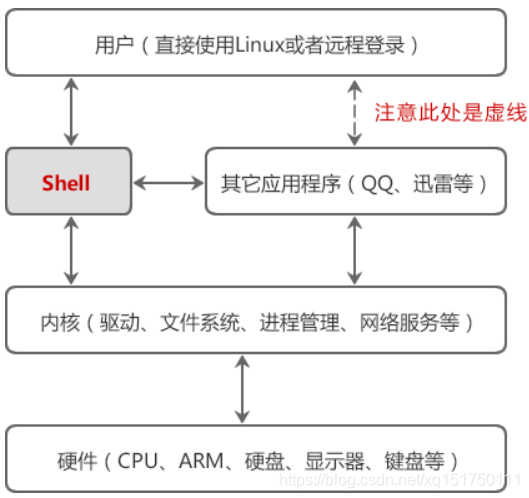
\includegraphics[width=0.7\textwidth]{shell.png}
    \caption{shell工作流程示意图} % 图片标题
    \label{fig:shell} % 图片标签,用于引用
\end{figure}

shell的一大特性就是它是一个应用程序,它连接了用户和 Linux 内核,让用户能够更加高效、安全、低成本地使用 Linux 内核。另一大特性是它是一个命令语言解释器,shell把我们在计算机上的操作或我们的命令,翻译为计算机可识别的二进制命令,传递给内核,以便调用计算机硬件执行相关的操作;计算机执行完命令后,再通过Shell翻译成自然语言,呈现在我们面前。同时,Shell 程序设计语言支持在高级语言里所能见到的绝大多数程序控制结构,比如循环,函数,变量和数组等等。

常见的shell有Bourne shell (sh), C shell (csh), Korn shell (ksh), Bourne Again shell(bash, sh 的扩展),zsh等等。

启动shell的方法有两种,一是进入linux控制台,二是使用终端(快捷键为ctrl+alt+t)

\subsubsection{简单的shell脚本}

shell

\textbf{新建一个shell脚本}

打开文本编辑器,新建一个文件 test.sh

\begin{tcode}
	vim test.sh
\end{tcode}

然后在shell脚本的第一行输入

\begin{tcode}
	#!/bin/bash
\end{tcode}

\#! 是一个约定的标记,它告诉系统这个脚本需要什么解释器来执行,即使用哪一种 shell。在第一行下面就可以用shell编程语言输入脚本内容了,以下是一个简单的例子:

\begin{tcode}
	#!/bin/bash
	echo "Hello World !"
\end{tcode}

shell脚本可用于ROS程序自启,即编写一系列命令行操作,启动程序时无需打开终端敲命令行,只需启动一个shell脚本即可。

\textbf{运行shell脚本}

运行shell脚本也有两种方式:

\begin{enumerate}
\item 作为可执行程序

先使脚本具有执行权限

\begin{tcode}
	chmod +x ./test.sh
\end{tcode}

再执行脚本

\begin{tcode}
	./test.sh
\end{tcode}

\item 作为解释器参数

直接运行解释器,其参数就是 shell 脚本的文件名。eg:

\begin{tcode}
	/bin/sh test.sh
	/bin/php test.php
\end{tcode}

这种方式运行的脚本,不需要在第一行指定解释器信息,写了也没用
\end{enumerate}

\subsubsection{linux中的bash}

根据刚刚对shell的介绍可以知道bash也是一种shell,事实上在大多数的linux系统中,bash是默认的缺省shell。当然如果你不想用bash也可以换成其他的shell(比如zsh也很好用)。

bash和shell一样有许多强大的功能,经常用到的有命令补全,通配符,命令历史记录,重定向,管道等等。bash的配置文件分为全局配置文件和个人配置文件:

\begin{center}
\textbf{bash主要文件}
	\begin{tabular}{cc}
		\toprule[1.5pt]
		文件 & 作用\\
		\midrule[1pt]
		$  /etc/profile    $		&系统的主配置文件,用于设置系统范围内的环境变量和其他系统的设置\\
		$  \texttildelow /.bashrc    $		&用于定义用户的命令别名和本地变量\\
		$  \texttildelow /.bash\_profile   $		&用于定义用户的环境变量,运行命令或脚本\\
		\bottomrule[1.5pt]
	\end{tabular}
\end{center}

其中我们会经常对.bashrc文件进行操作。

.bashrc是终端里面指令运行的配置脚本,是系统的隐藏文件,存放在\texttildelow 目录下。.bashrc的功能主要有两个:

\begin{enumerate}
\item 个性化指令alias:alias [指令别名]='原指令'

注意alias和=之间不能有空格

\item 设定环境路径:export PATH=\$PATH:路径
\end{enumerate}

对.bashrc中的内容进行修改后,在下一次打开新终端时修改内容才会生效,或执行source \texttildelow /.bashrc立刻生效。

\subsubsection{linux系统环境变量简介}

linux系统中有非常多的环境变量在控制系统的运行,常用的有:

\begin{enumerate}
\item PATH:决定了shell将到哪些目录中寻找命令或程序

\item HOME:当前用户主目录

\item SHELL:当前用户Shell类型
\end{enumerate}

这里我们主要介绍PATH环境变量

PATH说简单点就是一个字符串变量,当输入命令的时候linux会去查找PATH里面记录的路径,path 配置的路径下的文件可以在任何位置执行,并且可以通过which 可执行文件命令来找到该文件的位置。注意PATH是大写,linux中区分大小写。

我们先来查看一下PATH:

\begin{tcode}
	echo $PATH
\end{tcode}

终端中会输出

/usr/local/sbin:/usr/local/bin:/usr/sbin:/usr/bin:/sbin:/bin:/usr/games:

/usr/local/games:/usr/lib/wsl/lib:/snap/bin


每个路径中间用:隔开,输入命令时系统根据这些路径来寻找对应的可执行文件,先找到谁就用谁

设置环境变量的方法有两种:

\begin{enumerate}
\item export PATH=/bin:/sbin:/usr/bin:/usr/sbin

\item PATH="/bin:/sbin:/usr/bin:/usr/sbin"
\end{enumerate}

这两种方法都是将PATH环境变量设置为包含了/bin、/sbin、/usr/bin、/usr/sbin这四个目录,但不同在于第一个命令是将PATH变量设置为一个新的字符串,第二个命令则是将PATH变量设置为一个已经存在的字符串,会覆盖之前的设置。并且不用export设置的环境变量仅对当前shell起作用,不会传导到子进程,export设置的环境变量在子进程也有效,因此我们常用export命令来设置PATH环境变量。

修改环境变量的方法有三种:

\begin{enumerate}
\item 直接在终端输入

\begin{tcode}
	export PATH=/usr/local/mongodb/bin:$PATH
\end{tcode}

\$PATH表示在原有PATH的基础上继续在前面或后面添加相应路径,这样可以避免修改原有路径。由于是在终端中输入命令,因此这种修改方式仅对当前用户当前终端有效。

\item 修改.bashrc文件:在.bashrc文件中添加export PATH=/usr/local/mongodb/bin:\$PATH一行,保存退出后source或打开新终端即可生效。该方法对当前用户永久有效。

\item 修改/etc/profile文件:找到设置PATH的行,添加export PATH=/usr/local/mongodb/bin:\$PATH,系统重启或运行source /etc/profile后生效。由于是修改了整个系统的配置文件,因此该方法对所有用户永久有效。
\end{enumerate}

环境变量这里介绍的很浅,主要目的是让读者先对环境变量这个概念有所了解,在后续自己配环境的过程中逐步加深对环境变量的理解,避免对系统环境变量的误操作。

